The two microphone structures are fabricated on a silicon wafer on which an insulating layer has been grown. \\
On top of the insulating layer, the conductive backplate is deposited, and spacers to support the membrane are formed. \\
The lateral spacers must be non-conductive to prevent electrical shorting between the backplate and the diaphragm. \\
On top of the spacers, the membrane, made of aluminum, is placed.

\newpage
\noindent
The first structure has a perforated diaphragm and includes corrugations to facilitate membrane deflection in that region (\autoref{fig:perforated_diaphragm_cross_section}).

\begin{figure}[h!]
    \centering
    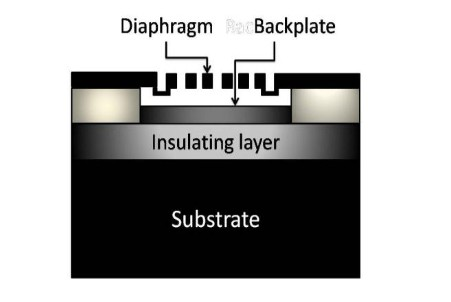
\includegraphics[width=0.7\linewidth]{img/perforated_diaphragm_cross_section.jpg}
    \caption{Cross section of capacitive microphone with corrugated and perforated diaphragm}
    \label{fig:perforated_diaphragm_cross_section}
\end{figure}

\noindent
The second structure has a corrugated membrane with no holes, but has a perforated backplate (\autoref{fig:perforated_backplate_cross_section}).

\begin{figure}[h!]
    \centering
    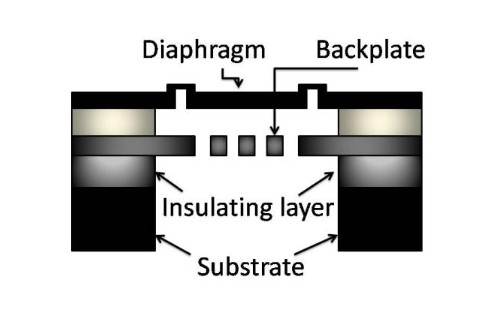
\includegraphics[width=0.7\linewidth]{img/perforated_backplate_cross_section.jpg}
    \caption{Cross section of capacitive microphone with perforated backplate}
    \label{fig:perforated_backplate_cross_section}
\end{figure}

\noindent
The main differences between these two structures are:

\begin{itemize}
    \item Air flows through the diaphragm holes in the first structure and through the backplate holes in the second structure.
    \item The perforated membrane is mechanically weaker than the solid one.
\end{itemize}

\noindent
As shown in \cite{jerman1986}, for shallow sinusoidal corrugations the deflection is approximately given by \cref{eq:diaphragm_deflection} \\

\begin{equation}
    \begin{cases}
        \frac{PR^4}{E'h^4} = a_p \frac{y}{h} + b_p \frac{y^3}{h^3} \\
        \\
        a_p = \frac{2(q+3)(q+1)}{3\left(1-\frac{v^2}{q^2}\right)} \\
        \\
        b_p = \frac{165(q+1)^3(q+3)}{q^2(q+4)(q+11)(2q+1)(3q+5)}
    \end{cases}
    \label{eq:diaphragm_deflection}
\end{equation}

\noindent
where:

\begin{itemize}
    \item \textbf{P}: Applied pressure
    \item \textbf{R}: Diaphragm radius
    \item \textbf{h}: Diaphragm thickness
    \item \textbf{y}: Diaphragm center deflection
    \item \textbf{v}: Poisson’s ratio
\end{itemize}

\noindent
The terms \(E^{'}\) and \(q\), for shallow sinusoidal profiles, are given by \cref{eq:E_param} and \cref{eq:q_param}:

\begin{equation}
    E^{'} = \frac{E}{1-v^2}
    \label{eq:E_param}
\end{equation}

\begin{equation}
    q = 1 + 1.5 \cdot \frac{H^2}{h^2}
    \label{eq:q_param}
\end{equation}

\noindent
where:

\begin{itemize}
    \item \textbf{E}: Young’s modulus
    \item \textbf{H}: Corrugation depth
\end{itemize}

\noindent
The approximated formula is more accurate for the perforated-backplate structure, because the membrane is corrugated without holes.
